\subsection{Persistencia}\label{sec:persistence}
La implementación del componente de persistencia se enfoca en dar servicio a los componentes de escritorio y web, por esta razón la implementación se ha dividido en dos partes:
\begin{enumerate}
 	\item Escritorio: la automatización de rutinas, dado que estas rutinas son ejecutadas dentro del ambiente de Sahi (que a su vez está en la plataforma de Java) se utiliza la biblioteca JDBC para economizar los recursos físicos del equipo del operador de la farmacéutica.
 	\item Web: generación de reportes, administración de órdenes de reposición, administración de catálogos y operaciones de identificación  de usuarios. Para esta parte se utilizó el marco de trabajo de Spring en conjunción con el marco de trabajo MyBatis (ver sección \ref{sec:mybatis}).
\end{enumerate}
Los siguientes apartados explican la implementación de los servicios para escritorio y web.

\subsubsection{Persistencia para funcionalidades de escritorio}
\paragraph{\indent Interfaz Almacenamiento\\}
Implementación de las operaciones para las rutinas de automatización que requieren almacenar o modificar datos, para simplificar la explicación se mostrarán ejemplos de la manipulación de datos en lugar de mostrar la implementación de cada operación de la interfaz:
\begin{enumerate}
	\item Inserción: la operación de inserción se ocupa en las operaciones \textbf{guardar-nueva} y \textbf{registrar-evento}, la inserción consiste de los siguientes puntos (en el Código \ref{lst:per-insert-order} se muestra la implementación de la operación \textbf{guardar-nueva}):
	\begin{enumerate}
		\item Plantilla de la sentencia SQL (línea 1).
		\item Creación de los objetos de la biblioteca JDBC (línea 4).
		\item Agregar datos específicos de la inserción (líneas 5 a 7).
		\item Ejecución de la sentencia (línea 8).
	\end{enumerate}

	\begin{lstlisting}[language=Java, caption={Inserción de una nueva orden de reposición en la base de datos.}, captionpos=b, label={lst:per-insert-order}]
private static final String INSERT_ORDEN = "INSERT INTO ordenes(contrato, solicitud, orden, fecha_expedicion, almacen_destino, url_con, url_env, estatus, id_sesion_insersion, id_sesion_estatus, fecha_estatus) VALUES(?, ?, ?, ?, ?, ?, ?, 1, ?, ?, CURRENT_TIMESTAMP)";

public void insertOrden(Orden orden) throws SQLException{
    try(PreparedStatement pst = conn.prepareStatement(INSERT_ORDEN)){
	    pst.setString(1, orden.getContrato());
	    ...
	    pst.setLong(9, orden.getIdSesionInsersion());
	    pst.executeUpdate();
	}
}
	\end{lstlisting}

	\item Actualización: la actualización de datos es utilizada por las operaciones \textbf{cambiar-estado}, \textbf{guardar-respuesta}, \textbf{guardar-folio-acuse} y \textbf{actualizar-estado-sa}, la actualización consiste de los siguientes puntos (en el Código \ref{lst:per-update-status} se muestra la implementación de la operación \textbf{cambiar-estado}):
	\begin{enumerate}
		\item Plantilla de la sentencia SQL, línea 1 del Código \ref{lst:per-update-status}.
		\item Creación de los objetos de la biblioteca JDBC, línea 4 del Código \ref{lst:per-update-status}.
		\item Agregar datos de la actualización, líneas 5 a 8 del Código \ref{lst:per-update-status}.
		\item Ejecución de la sentencia, línea 9 del Código \ref{lst:per-update-status}.
	\end{enumerate}

	\begin{lstlisting}[language=Java, caption={Actualización del estado de una orden de reposición.}, captionpos=b, label={lst:per-update-status}]
private static final String UPDATE_STATUS = "UPDATE ordenes SET estatus = ?, fecha_estatus = CURRENT_TIMESTAMP, id_sesion_estatus = ? WHERE contrato = ? AND orden = ?";

private void updateEstatus(Orden orden) throws SQLException{
	try(PreparedStatement pst = conn.prepareStatement(UPDATE_STATUS)){
		pst.setInt(1, orden.getEstatus());
		pst.setLong(2, orden.getIdSesionEstatus());
		pst.setString(3, orden.getContrato());
		pst.setLong(4, orden.getOrden());
		pst.executeUpdate();
	}
}
	\end{lstlisting}
\end{enumerate}

\paragraph{\indent Interfaz Lectura\\}
Implementación de las operaciones para las rutinas de automatización que tienen como objetivo la obtención de datos, esto no quiere decir que durante el llamado de estas operaciones no se modifiquen datos.
Dado que la obtención de los datos se convierte a objetos del dominio del proyecto AutoSA. Se ha implementado una solución basada en los patrones de diseño Estrategia (ver Apéndice \ref{sec:strategy}) y Singleton (ver Apéndice \ref{sec:singleton}). \\
En la Figura \ref{fig:dia-class-mapper} se el diagrama de clases de la solución:
\begin{figure}[h]
	\centering
	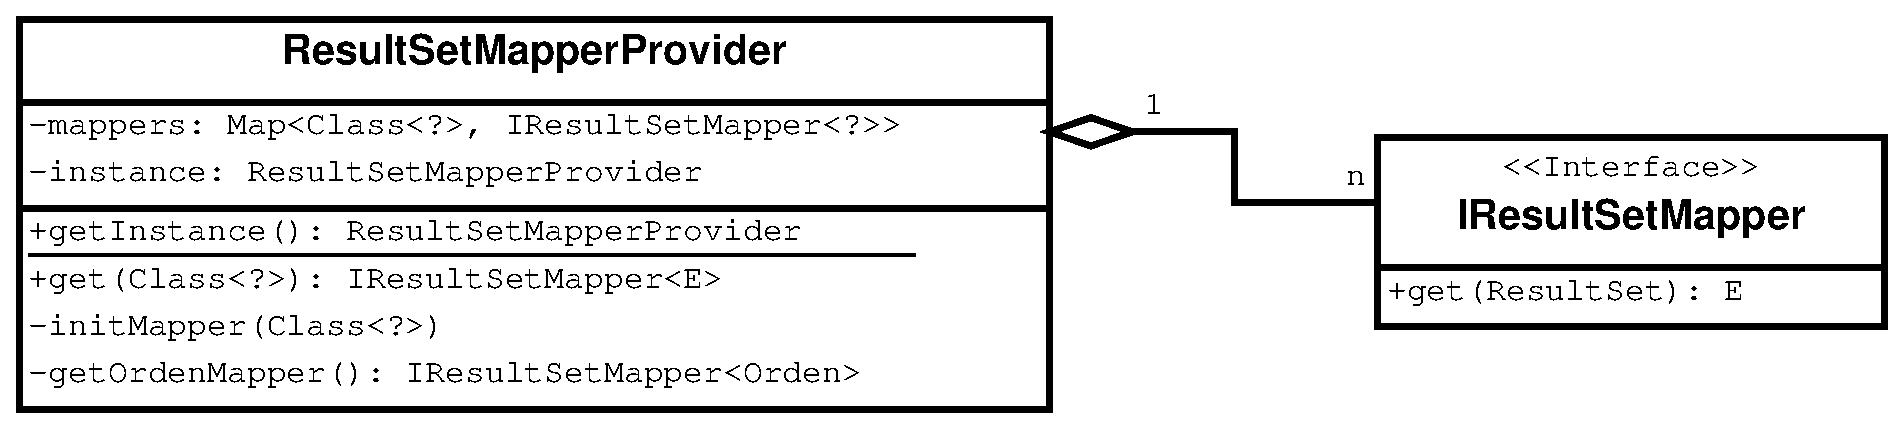
\includegraphics[width=\textwidth]{dia-class-mapper}
	\caption{Diagrama de clase de ResultSetMapperProvider.}
	\label{fig:dia-class-mapper}
\end{figure}

La clase \textbf{IResultSetMapper} tiene como función la conversión de la información obtenida por la biblioteca JDBC de la base de datos a objetos del dominio del proyecto AutoSA. El Código \ref{lst:per-i-rs-mapper} muestra la definición de la interfaz de Java.
	\begin{lstlisting}[language=Java, caption={Interfaz IResultSetMapper.}, captionpos=b, label={lst:per-i-rs-mapper}]
public interface IResultSetMapper<E>{
	E get(ResultSet resultSet) throws SQLException;
}
	\end{lstlisting}

La clase \textbf{ResultSetMapperProvider} es la encargada de la construcción y administración de las clases del tipo \textbf{IResultSetMapper}.\\
El Código \ref{lst:per-class-mapper-provider} muestra la declaración del la clase \textbf{ResultSetMapperProvider} donde se observa el uso del patrón de diseño Singleton:
\begin{enumerate}
	\item Línea 3, instancia privada de la clase.
	\item Línea 5, constructor de clase privado.
	\item Línea 9, método para obtener la instancia de clase.
\end{enumerate}

\begin{lstlisting}[language=Java, caption={Clase ResultSetMapperProvider con patrón de diseño Singleton.}, captionpos=b, label={lst:per-class-mapper-provider}]
public class ResultSetMapperProvider{
	private final Map<Class<?>, IResultSetMapper<?>> mappers;
	private static ResultSetMapperProvider instance;
	
	private ResultSetMapperProvider(){
		mappers = new LinkedHashMap<Class<?>, IResultSetMapper<?>>();
	}
	
	public static ResultSetMapperProvider getInstance(){
		if(instance == null){
			instance = new ResultSetMapperProvider();
		}
		return instance;
	}

	public <E> IResultSetMapper<E> get(Class<?> beanType){...}
	private void initMapper(Class<?> beanType){...}
	private IResultSetMapper<Orden> getOrdenMapper(){...}
}
\end{lstlisting}

La clase \textbf{ResultSetMapperProvider} realiza la construcción de los objetos del tipo \textbf{IResultSetMapper} como se muestra en el Código \ref{lst:per-get-orden-mapper}:
\begin{lstlisting}[language=Java, caption={}, captionpos=b, label={lst:per-get-orden-mapper}]
private IResultSetMapper<Orden> getOrdenMapper(){
	return new IResultSetMapper<Orden>(){
		public Orden get(ResultSet rs) throws SQLException{
			Orden orden = new Orden();
			orden.setId(rs.getLong("id"));
			...
			return orden;
		}
	};
}
\end{lstlisting}

La clase \textbf{ResultSetMapperProvider} da acceso a las instancias de tipo \textbf{IResultSetMapper} mediante el método \textbf{get} como se muestra en las líneas 1 a 6 del Código \ref{lst:per-get-rs-mapper}, si no se encuentra una instancia para la clase solicitada, entonces se crea como se muestra en las líneas 2 a 4 y 8 a 20 del Código \ref{lst:per-get-rs-mapper}
\begin{lstlisting}[language=Java, caption={Obtención de instancias de IResultSetMapper.}, captionpos=b, label={lst:per-get-rs-mapper}]
public <E> IResultSetMapper<E> get(Class<?> beanType){
	if(!mappers.containsKey(beanType)){
		initMapper(beanType);
	}
	return (IResultSetMapper<E>)mappers.get(beanType);
}

private void initMapper(Class<?> beanType){
	if(Orden.class.equals(beanType)){
		mappers.put(beanType, getOrdenMapper());
	}else if(OrdenPemex.class.equals(beanType)){
		mappers.put(beanType, getPemexMapper());
	}else if(ProductoPemex.class.equals(beanType)){
		mappers.put(beanType, getProductoPemexMapper());
	}else if(Sesion.class.equals(beanType)){
		mappers.put(beanType, getSesionMapper());
	}
}
\end{lstlisting}

La solución anterior lleva a la implementación de las operaciones de la interfaz ``Lectura'':
\begin{enumerate}
	\item \textbf{siguiente-orden-contestar}, \textbf{siguiente-orden-enviar} y \textbf{obtener-datos-acuse}: todas las operaciones de lectura siguen los mismos pasos (en el Código \ref{lst:per-next-orden} se muestra la implementación de la operación \textbf{siguiente-orden-contestar}):
	\begin{enumerate}
		\item Plantilla de la sentencia SQL, línea 1 del Código \ref{lst:per-next-orden}.
		\item Creación de los objetos de la biblioteca JDBC, línea 4 del Código \ref{lst:per-next-orden}.
		\item Realizar la consulta a la base de datos, línea 6 del Código \ref{lst:per-next-orden}.
		\item Lectura del resultado de la consulta, líneas 7 a 9 del Código \ref{lst:per-next-orden}.
	\end{enumerate}

	\begin{lstlisting}[language=Java, caption={Lectura de una orden de reposición desde la base de datos.}, captionpos=b, label={lst:per-next-orden}]
private static final String NEXT_TO_MANAGE = "SELECT * FROM ordenes WHERE estatus = ? ORDER BY fecha_insersion LIMIT 1";

public Orden getNextOrden(Integer estatus) throws SQLException{
	try(PreparedStatement pst = conn.prepareStatement(NEXT_TO_MANAGE)){
		pst.setInt(1, estatus);
		try(ResultSet rs = pst.executeQuery()){
    		if(rs.next()){
    			IResultSetMapper<Orden> mapper = ResultSetMapperProvider.getInstance().get(Orden.class);
    			return mapper.get(rs);
    		}
		}
	}
	return null;
}
	\end{lstlisting}
\end{enumerate}

\subsubsection{Persistencia para funcionalidades Web}\label{sec:persistence-web}
La interfaz del componente Persistencia dedicado a las funcionalidades ofrecidas mediante la interfaz web utiliza MyBatis cuya implementación sigue los pasos mencionados en la sección \ref{sec:mybatis}.\\
\indent 1. En el Código \ref{lst:per-batis-config} se muestra la configuración del objeto \textbf{SqlSessionFactoryBean}: 
\begin{enumerate}
	\item Habilitar contexto para transacciones (Línea 1).
	\item Crear los objetos para manejar la persistencia (Línea 2).
	\item Lectura de las interfaces para crear los objetos de persistencia (Línea 3).
\end{enumerate}
\begin{lstlisting}[language=XML, caption={Configuración de MyBatis con Spring.}, captionpos=b, label={lst:per-batis-config}]
<tx:annotation-driven />
<bean id="sqlSessionFactory" class="org.mybatis.spring.SqlSessionFactoryBean">
	<property name="dataSource" ref="dataSource" />
	<property name="mapperLocations" value="classpath:com/surtimiento/persistence/dao/*.xml" />
</bean>
<mybatis:scan base-package="com.surtimiento.persistence.dao"/>
\end{lstlisting}

\indent 2. El Código \ref{lst:per-batis-user} muestra la configuración para el manejo de usuarios de la interfaz web:
\begin{enumerate}
	\item Relación entre tabla de roles y clase Rol.
	\item Relación entre tabla de usuarios y clase de Usuario.
	\item Consulta SQL para obtener un usuario.
\end{enumerate}
\begin{lstlisting}[language=XML, caption={Definición de relación de MyBatis.}, label={
lst:per-batis-user}]
<mapper namespace="com.meve.surtimiento.persistence.dao.IDomainUser">
  <resultMap id="rol" type="com.meve.surtimiento.domian.RolDomain" autoMapping="true">
    <id property="rol" column="rol"/>
  </resultMap>
  <resultMap id="usuario" type="com.meve.surtimiento.domian.UsuarioDomain" autoMapping="true">
    <id property="usuario" column="usuario"/>
    <collection property="roles" resultMap="rol" javaType="ArrayList"/>
  </resultMap>
  <select id="getUsuario" resultMap="usuario" useCache="false">
    SELECT u.*, r.*
      FROM usuarios u, roles_domain r, usuarios_roles ur
     WHERE u.usuario = ur.usuario AND r.rol = ur.rol AND u.usuario = #{0};
  </select>
</mapper>
\end{lstlisting}

\indent 3. Por último se el Código \ref{lst:per-batis-user-interface} muestra la interfaz de Java para utilizar las consultas del paso anterior.
\begin{lstlisting}[language=Java, caption={Interfaz de Java para la fábrica de MyBatis.}, captionpos=b, label={lst:per-batis-user-interface}]
public interface IDomainUser{
	UsuarioDomain getUsuario(String name);
}
\end{lstlisting}
